\chapter{The justificatory structure of OWL ontologies}
\label{chap:structure}

In current ontology explanation tools, justifications are generally represented as individual entities in relation to a single entailment. However, this view neglects the rich relations that can be found between \emph{multiple} justifications for both single and multiple entailments of OWL ontologies. Previous surveys of OWL ontologies have shown that the majority of ontologies used in practice contain some entailment which has more than one justification, with many ontologies generating a few dozen and up to several hundred justifications for a single entailment \cite{bail10kb,horridge11ab,bail11jm}. 

Several properties of justifications, such as the number of justifications for an entailment, the size of justifications in an ontology, to which extent the ontology contains entailments which are entailed only by themselves, and which proportion of the ontology participates in justifications, all give us an insight into structural relationships in the ontology beyond standard metrics; we can say that the justifications make the \emph{implicit} relationships between the entitites and axioms of an ontology \emph{explicit}.

Further, justifications for a single or multiple entailments are not disjoint subsets of an ontology, but they often \emph{overlap} to a certain extent, sharing one or more axioms between them. This is relevant for both understanding as well as repairing the entailments of such justifications: shared axioms may\footnote{It is important to point out that a shared axiom does \emph{not} necessarily have to be an incorrect axiom; therefore, it is not guaranteed to be part of the hitting set that leads to a repair.} lead to a smaller hitting set, and therefore to a smaller repair for a set of entailments. Further, shared axioms may indicate common lemmas \cite{horridge09ct}, i.e.\ intermediate entailments, which can assist users in understanding (parts of) multiple justifications at the same time rather than treating each one independently, thus reducing the effort required to deal with multiple justifications.

In this chapter, we will introduce the notion of \emph{justificatory structure} of an OWL ontology. First, we present a categorisation of entailments based on the types of justifications they have in an ontology. We then lay out the motivation for analysing the relations between justifications in an ontology and define various structural aspects which may be of interest for ontology development and analysis. We introduce a graph-based representation of the justifications and entailments in an ontology and describe the generation and implementation of such a \emph{j-graph}. Along with Chapter 5, the work presented in this chapter constitutes the core of our research into the justificatory structure of OWL ontologies.


\section{Categories of justifications and entailments}
Following on from our discussion of different entailment sets in the previous chapter, we will now take a closer look at the different types and scenarios of justifications we encounter when analysing a finite entailment set of an ontology. While it is certainly the case that justifications are essentially equal---they are minimal entailing axiom subsets---we may treat them differently depending on the axioms they contain, and depending on their relation to the entailment in question.

\subsection{Self-justifications and self-supporting entailments}
Any justification which is simply the entailed axiom itself is classified as a \emph{self-justification}:
\begin{defn}[Self-justification]
A justification \J for an entailment \ent is a \emph{self-justification} if \J = $\{\eta\}$.
\end{defn}
We distinguish between entailments which have a self-justification in addition to other, more complex, justifications, and entailments which have \emph{only} a self-justification and no other justifications. Referring back to our discussion of finite entailment sets in Chapter 3, these entailments are commonly referred to as \enquote{asserted, but not inferred}; however, in order to avoid ambiguity caused by the word \emph{inferred} (as an asserted axiom can also be inferred from an ontology), we denote such as \emph{self-supporting} entailments: 
\begin{defn}[Self-supporting entailment]
An entailment \ent is \emph{self-supporting} if $\justseta = \{\{\eta\}\}$.
\end{defn}
There are different reasons why an entailment might have a self-justification \emph{in addition} to other justifications: 
\begin{compactenum}
\item The entailment was not asserted in the ontology to begin with, but explicitly added after it was found to be inferred. This could be in order to improve reasoner performance, to make the entailment visible to the \emph{developer} without using a reasoner (e.g.\ if the classification time is very high), or to make the inferences visible to \emph{end-users} in an ontology browser interface which does not support reasoning. 
\item The ontology modeller does not use a reasoner during the engineering process, thus is not aware that the subsumption is already entailed by the ontology, which means they might explicitly assert information which already exists implicitly.
\item The additional justifications are a side-effect of other axioms that were added to the ontology without the aim of causing the entailment, or with the aim of causing this \emph{and}  other entailments.
\end{compactenum}
Without additional information, such as axiom annotations or change logs of an ontology, it is not possible to tell the intentions of an ontology developer when adding an axiom which causes additional justifications or self-justifications. Moreover, developers may not even be \emph{aware} of the full impact that a modification has on the ontology. We therefore treat self-justifications and additional justifications on a purely logical level, disregarding the reasons for those multiple justifications.


\subsection{Atomic subsumption chains}

An \emph{atomic subsumption chain justification} in an ontology \O is a set of axioms of the type \dlax{A_{1} \subcls A_{2}},  \dlax{A_{2} \subcls A_{3}}, \ldots,  \dlax{A_{n-1} \subcls A_{n}} for an entailment \dlax{A_{1} \subcls A_{n}} where \dlcn{A_{i}} is a named class in \sig{\O}. It is clear to see that such an atomic subsumption chain justification of two or more axioms always represents an \emph{indirect} subsumption, which we have discussed in Chapter 3. Take, for example, the following ontology:
\begin{examp}
\begin{align*}
\O = \{ \dlax{A \subcls B}, \dlax{B \subcls C}, \dlax{A \subcls C} \}
\end{align*}
\end{examp}
The $A^{+}D^{-}$ entailment set of atomic subsumptions is the set $\{\dlax{A \subcls B}, \dlax{B \subcls C} \}$, whereas the  $(AD)^{+}$ entailment set is simply \O itself. While each entailment in $(AD)^{+}$ has a self-justification, the entailment \dlax{A \subcls C} has an additional atomic subsumption chain justification $\J=\{ \dlax{A \subcls B}, \dlax{B \subcls C} \}$. Despite \J being slightly less trivial than a self-justification, it is still simply based on the transitivity of subsumption. This implies that the interactions between axioms in the ontology (with respect to the class hierarchy) are trivial enough to be inferred by a structural reasoner.

Note that it is certainly possible for an entailment to have multiple atomic subsumption chain justifications. For example, adding the axioms $\{\dlax{A \subcls E}, \dlax{E \subcls C} \}$ to the above example would add another atomic subsumption chain justification for the entailment \dlax{A \subcls C}. 

In our survey of the justificatory structure of OWL ontologies presented in Chapter \ref{chap:survey}, we find that many ontologies which only contain self-justifications for direct subsumptions often have only atomic subsumption chain justifications for indirect subsumptions; that is, the information content of the ontology does not reach beyond its asserted class graph. 

\subsection{Complex justifications}
\label{sec:complexjusts}

Finally, we consider all justifications that are not self-justifications or atomic subsumption chains to be \emph{complex} justifications as opposed to \emph{trivial} self-justifications or atomic subsumption chain justifications. It is obvious that the level of complexity can vary strongly between justifications, depending on their size and the constructors used in their axioms. However, for the purpose of categorising justifications, such a coarse distinction between self-justifications, atomic subsumption chains, and \emph{other} justifications suffices.

It is clear to see that entailments can have both trivial and complex justifications. Assume we add further axioms to the above example ontology \O to obtain $\O' = \O \cup \{ \dlax{A \subcls \exists r.D, \exists r.D \subcls C}\}$. The entailment \dlax{A \subcls C} will then have another, complex, justification $\J = \{ \dlax{A \subcls \exists r.D, \exists r.D \subcls C}\}$ in addition to its self-justification and atomic subsumption chain justification.


\subsection{Categorising entailments and ontologies}

If we consider the categorisation of justifications from the point of view of their corresponding entailments, we can also arrange entailments and ontologies into a hierarchy based on their justification. This will be of use when analysing the justificatory structure of an ontology, as it allows us to decide which entailments and justifications to include in specific metrics. For example, when counting the numbers of justifications per entailment, we may want to treat trivial and non-trivial justifications separately in order to ensure that we are comparing equally relevant justifications. 

\begin{figure}
\centering
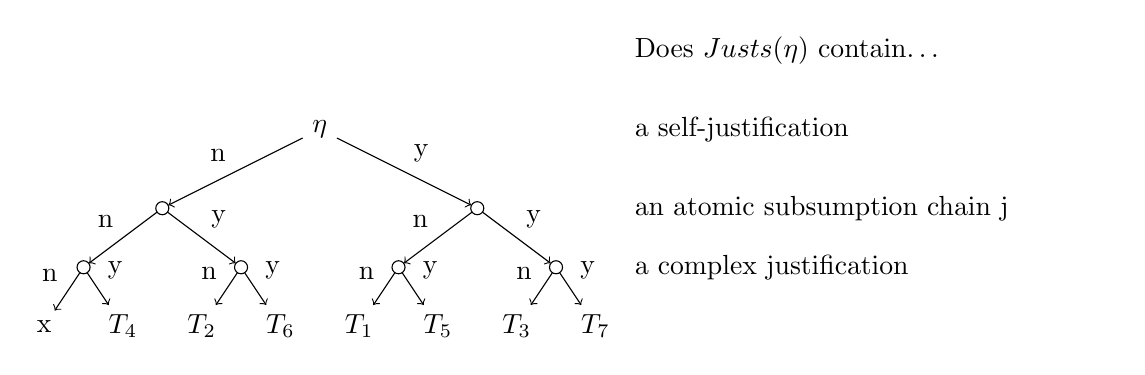
\begin{tikzpicture}[scale=1,->,auto=left]
  
%  \draw (-2,8.25) -- (6,8.25) -- (6,7.75) -- (-2,7.75) -- cycle;
% \draw (-2,7.5) -- (6,7.5) -- (6,7) -- (-2,7) -- cycle;
%  \draw (-2,8.25) -- (6,8.25) -- (6,7.75) -- (-2,7.75) -- cycle;
\node[align=left,text width=6cm] at (9,10) {Does $Justs(\eta)$ contain\ldots};
\node[align=left,text width=6cm] at (9,9) {a self-justification};
\node[align=left,text width=6cm] at (9,8) {an atomic subsumption chain j};
\node[align=left,text width=6cm] at (9,7.25) {a complex justification};
  
\node[draw=none] (root) at (2,9) {$\eta$};

\tikzstyle{every node} = [color=black,shape=circle,scale=0.5,draw]
  
\node (n) at (0,8)  {};
\node (y) at (4,8)  {};
\node (nn) at (-1,7.25)  {};
\node (ny) at (1,7.25)  {};
\node (yn) at (3,7.25)  {};
\node (yy) at (5,7.25)  {};

\tikzstyle{every node} = [draw=none]
\node[draw=none] (nnn) at (-1.5,6.5)  {x};

\node (nny) at (-0.5,6.5)  {$T_{4}$};	
\node (nyn) at (0.5,6.5)  {$T_{2}$};
\node (nyy) at (1.5,6.5)  {$T_{6}$};
\node (ynn) at (2.5,6.5)  {$T_{1}$};
\node (yny) at (3.5,6.5)  {$T_{5}$};
\node (yyn) at (4.5,6.5)  {$T_{3}$};
\node (yyy) at (5.5,6.5)  {$T_{7}$};



\draw (root) to node [swap]  {n} (n);
\draw (root) to node {y} (y);

\draw (n) to node [swap] {n} (nn);
\draw (n) to node {y} (ny);

\draw (nn) to node [swap]  {n} (nnn);
\draw (nn) to node {y} (nny);

\draw (ny) to node [swap]  {n} (nyn);
\draw (ny) to node {y} (nyy);

\draw (y) to node [swap]  {n} (yn);
\draw (y) to node {y} (yy);

\draw (yn) to node  [swap] {n} (ynn);
\draw (yn) to node  {y} (yny);

\draw (yy) to node [swap]  {n} (yyn);
\draw (yy) to node  {y} (yyy);


\end{tikzpicture}
\caption{A decision tree for categorising entailments.}
\label{fig:entailmenthierarchy}
\end{figure}

Figure \ref{fig:entailmenthierarchy} shows a decision tree for categorising an entailment based on its justifications. Given an entailment, the decision tree accepts a simple yes/no in the presence/absence of each type of justification, leading the entailment to be sorted into one of seven categories. We have labelled these categories with types $T_{1}$ through $T_{7}$ based on the number obtained if we regard the respective path in the decision tree as a (reversed) binary number. This results in uneven numbers for entailments which have self-justifications, and even numbers for those entailments that have only non self-justifications. 

This categorisation process can be applied to ontologies in order to rank them based on the justification types they contain (given some finite entailment set). This is of use when analysing the justificatory structure of an ontology, as it allows us to separate relevant ontologies (those that do contain entailments with complex justifications) from irrelevant ones (those that only contain trivial entailments). 



\section{Representing justifications as j-graphs}

In order to talk about the justificatory structure of an ontology, we require some way of representing structural aspects in an accessible way. The set of entailments, their justifications, and the axioms occurring in these justification can be easily represented as a graph, which allows us to describe aspects of justificatory structure using standard graph metrics such as the in- and out-degrees of nodes. In this section, we first define the terminology for different aspects of entailment and justification sets, which then allows us to define the \emph{justification graph} for a given set of entailments.


\subsection{J-graph definition}

Before defining j-graphs, we need to introduce the building blocks of these graph representations of justifications. Recall the notion of \justs which refers to the set of all justifications for the entailments in a particular finite entailment set of an ontology \O. Further, we define the set of all axioms occurring in all justifications for a particular entailment set:
\begin{defn}[Justification axioms]
\begin{align*}
\justax = \{\alpha \mid there~is~a~ \just \in \justs ~s.t.~\alpha \in \just\}
\end{align*}
\end{defn}
Based on our definitions of justification sets and justification axioms, we can now define the justification graph of an ontology \ont with respect to an entailment set \entset. A justification graph (\emph{j-graph}) \jgraph is a directed graph whose set of nodes is the union of the set of axioms \entset which are entailed by \O and the set \justax of axioms that participate in justifications for these entailments, together with the set of all justifications \justs. The graph does not contain axioms in \ont which are neither in the entailment set, nor in \justax, as these would not have any incoming or outgoing edges, thus not adding any information content.
\begin{defn}[Justification graph]
Given a set of entailments \entset, their justifications \justs, and justification axioms \justax, a \emph{justification graph} is a graph \jgraphdef where
\begin{compactitem}
\item $E_{1} =\{ (u,v) \in \entset \cup \justax \times \justs \mid u \in v\}$  and\\
\item $E_{2} =\{ (v,w) \in \justs\times \entset \mid v \in Justs(\ont, w) \}$.
\end{compactitem}
\end{defn}

\begin{figure}
\centering
\includedot[scale=0.6]{img/jgraph-example}
\caption{An example of a j-graph for justifications and entailments.}\label{fig:jgraphexample}
\end{figure}
Figure \ref{fig:jgraphexample} shows a j-graph of the small sample entailment and justification set in Example \ref{ex:jgraph}. As we can see in the example graph on nodes $a1$, $a10$, $a11$ and $a12$, an axiom node in the graph with an in-degree $\geq 1$ corresponds to an entailment in \entset. An axiom node with an out-degree $\geq 1$ correspond to an axiom in \justax; this node type is represented by nodes $a1$ through $a9$ in the example graph.

\begin{examp}\label{ex:jgraph}
\begin{align*}
j1 =& \{a1\} \models a1 \\
j2 =& \{a2, a3, a4\} \models a10\\
j3 =& \{a4, a5\} \models a11 \\
j4 =& \{a6, a7, a8\} \models a12\\
j5 =& \{a7, a8, a9\} \models a12\\
j6 =& \{a11\} \models a11
\end{align*}
\end{examp}

A self-justification corresponds to a cycle between an axiom node and a justification node (which, in turn, only has this one incoming edge), as justifications $j1$ and $j6$ show. A self-supporting entailment ($a1$ in the example graph) is represented by an axiom node which has no other incoming edges in addition to the cycle. 

Note that, while some j-graphs may be tripartite, an axiom node can be both in the set \justax and in \entset, i.e. have an outgoing edge to a justification node and an incoming edge from a justification node, as we can see from both axioms $a1$ and $a11$ in the example graph. Thus, a j-graph is bipartite, but not guaranteed to be tripartite.

There exists a \emph{unique} j-graph for every set of entailments, as the set of justifications for an entailment set is unique in an ontology, and the edges in the j-graph follow from these unambiguous relations.

Recall that the number of justifications for an entailment can potentially be exponential in the number of axioms in \ont. This affects the completeness of a j-graph for a given finite entailment set, as it may not be practical to compute \emph{all} justifications for \emph{all} entailments in the set. Despite the general feasibility of computing justifications, as shown in \cite{horridge11ab}, computing all justifications for a large finite entailment set can still require more time than an ontology user may consider practical. 

This means that we either need to sample a subset of entailments, or only generate a certain number of justifications for each entailment in the given entailment set---or both. While this omission of information is obviously problematic for users attempting to find a repair for \emph{all} justifications for a given entailment set, the only solution to such computational problems is incremental repair. Therefore, we only consider the j-graph for an entailment set to represent the particular set of entailments and justifications that could be processed, even if these are not all that exist in the ontology.


\subsection{J-graph generation}

\paragraph{Construction}

Generating a j-graph to represent the justificatory structure of an OWL ontology is a fairly straightforward process. First, all axioms in the union of the ontology and the selected entailment set \entset are labelled with a unique identifier $a_{i}$. We then compute the justifications for the entailments in \entset; the justifications are also labelled with unique identifiers $j_{k}$. The axiom labelling can also be performed on an existing set of justifications, which has no effect on the general structure of the process.

The j-graph is then constructed as follows: generate a node for each axiom in \justax and \entset (each justification in \justs) and label it with the respective identifier. For each justification node labelled $j_{k}$, generate an edge $(a_{i}, j_{k})$ for each axiom $a_{i}$ in the justification labelled $j_{k}$; this will create the edges representing the relation \enquote{axiom is used in justification}. For each entailment node $a_{i}$ with a justification $j_{k}$, generate an edge $(j_{k}, a_{i})$ which represents the relation \enquote{justification for entailment}. This construction requires only a single pass over all given justifications, axioms, and entailments.

	
\paragraph{Implementation}
\label{sec:jstrucimpl}
The above algorithm has been implemented using the OWL API version 3.2.4, and the JGraphT\footnote{\url{http://jgrapht.org/}} version 0.8.3 graph library for representing the j-graph. Construction of the graph on a set of existing justifications and entailments is performed quickly, with the average time to construct a graph being less than 10 seconds in a set of ontologies ranging from 2 to approximately 11,000 justifications.

%This concludes the introduction of the j-graph structure for representing justifications. Note that a graph representation may also lend itself as the basis justification-based interaction tool, since OWL users may already be familiar with graph-based ontology interaction tools, such as the OWLViz\footnote{\url{http://www.co-ode.org/downloads/owlviz/}} \protege plug-in.


\section{Justificatory structure}

Using the j-graph to describe relations between entailments, their justifications, and the axioms in the justifications, we can now discuss the various facets of the \emph{justificatory structure} of an OWL ontology. In a first instance, the justificatory structure provides additional ontology metrics; beyond these metrics, insights into the structure can support user understanding when coping with multiple justifications and/or multiple entailments. Further, in Chapter \ref{chap:understanding} we will introduce debugging techniques that are directly based on the interaction with the j-graph for a user-defined entailment set. 

Note that in this section we refer to \enquote{the entailments} and \enquote{the justifications} of an ontology, which requires a more precise specification. In what follows, we assume these entailments to be the $(AD)^{+}$ set of entailments which includes all asserted and inferred native, direct and indirect (non-tautologic) atomic subsumptions of the type \dlax{A \subcls B} for satisfiable classes $A, B$ which are entailed by \O, as this provides a clearly defined and natural starting point for exploring the properties of an ontology.

For ease of reading, we will use the terms \emph{justification}, \emph{axiom}, and \emph{entailment} interchangeably with \emph{justification node}, \emph{axiom node}, and \emph{entailment node} in the remainder of this chapter.

\subsection{Axiom properties}
\label{sec:arity}
The axioms occurring in justifications for a given set of entailments can have different properties, which we denote as axiom \emph{frequency}, \emph{impact}, and \emph{semantic relevance}. These three terms describe similar, but slightly distinct, measures of the effect an axiom in \justax has on a set of justifications and entailments. Figure \ref{fig:jgraph-arity} shows an example j-graph which exhibits different values of frequency, impact, and semantic relevance for the axiom node $a0$. Blank nodes labelled with \enquote{\ldots} indicate the existence of some additional axiom(s) occurring in a justification, respectively additional justification(s) for an entailment.

\begin{figure}
\centering
\includedot[scale=0.6]{img/jgraph-arityimpactsr}
\caption[J-graph illustrating axiom frequency, impact, semantic relevance.]{J-graph illustrating axiom frequency, impact, and semantic relevance. Axiom $a0$ has a frequency of 4, impact of 5, and semantic relevance of 3.} \label{fig:jgraph-arity}
\end{figure}

\subsubsection{Frequency}

The \emph{frequency}, also referred to as \emph{power} or \emph{arity}, of an axiom is the number of justifications (for a given entailment set \entset) the axiom occurs in. Removing an axiom with frequency $n$ from the ontology will break $n$ justifications for the entailments in \entset. Given that there can exist multiple justifications for an entailment, the frequency of the axioms in a set of justifications does not necessarily tell us how a removal would affect the actual \emph{entailments} of those justifications. In a j-graph, the frequency of an axiom node corresponds to its out-degree; an axiom with a frequency greater than 1 corresponds directly to a justification overlap of size 1 between the justifications the axiom occurs in:
\begin{defn}[Frequency]
$freq(u) =  \left|\lbrace v \mid  (u, v) \in E_{1}\rbrace \right|$ for $u \in \justax$.
\end{defn}
The axiom node $a0$ in Figure \ref{fig:jgraph-arity} has edges to four justifications ($j1$, $j2$, $j3$, $j4$); thus, $a0$ has a frequency of 4.

\subsubsection{Impact}

The \emph{impact} of an axiom is, in some sense, an extension of the axiom frequency. It refers to the number of \emph{entailments} in \entset that are directly affected by the axiom, as the axiom occurs in some justification for the entailments. Removing an axiom with an impact of $m$ from the ontology \emph{may} break $m$ entailments in \entset, assuming there are no other justifications for those $m$ entailments. Axiom frequency and impact coincide if each justification that the axiom occurs in has exactly one (distinct) entailment, and the impact is \emph{less} than the axiom frequency if the axiom occurs in multiple justifications for the same entailment. 

In a j-graph, the impact of an axiom node $u$ is defined as the sum of entailment nodes $w$ that  have an incoming edge from a justification node $v$ such that $(u, v) \in E_{1}$ and $(v, w) \in E_{2}$:
\begin{defn}[Impact]
$impact(u) =  \left| \lbrace w \mid  \exists v, w ~ s.t. ~ (u, v) \in E_{1}, (v, w) \in E_{2}\rbrace \right|$ for $u \in \justax$.
\end{defn}
The axiom node $a0$ in the j-graph in Figure \ref{fig:jgraph-arity} has an impact of 5, as it occurs in the justifications ($j1$, $j2$, $j3$, $j4$) for all five distinct entailments in the graph.

In the context of repairing a given set of entailments, we will need to consider the impact of axioms both with regard to the set of \emph{unwanted} as well as the set of \emph{wanted} entailments: removing a high-impact axiom from an ontology may break a large number, or all, unwanted entailments (e.g.\ unsatisfiable classes), but it may also lead to the removal of relevant information. Referring to our definitions of wanted and unwanted entailment sets in Section \ref{sec:wantedunwanted}, we can distinguish between the \emph{positive} and \emph{negative} impact of an axiom:
\begin{defn}[Positive and negative impact]
\begin{align*}
impact^{-}(\alpha) &= \left| \{\eta_{i} \mid \eta_{i} \in \entsetplus, \alpha \in JustAx(\entsetplus)\}\right| \\\
impact^{+}(\alpha) &= \left| \{\eta_{i} \mid \eta_{i} \in \entsetminus, \alpha \in JustAx(\entsetminus)\} \right| \\\
\end{align*}
\end{defn}	
In words, the negative impact of an axiom $\alpha$ is the number of \emph{wanted} entailments that are entailed by the justifications $\alpha$ occurs in, and the positive impact is the number of \emph{unwanted} entailments that are entailed by the justifications $\alpha$ occurs in. Note that the plus and minus signs for positive/negative impact and wanted/unwanted entailment sets are swapped, i.e. $impact^{-}$ refers to \entsetplus, and vice versa.

\subsubsection{Semantic relevance}
Finally, the \emph{semantic relevance} of an axiom, as defined by Kalyanpur \cite{kalyanpur06nm},  is the number of entailments that are \emph{dependent} on the axiom. Semantic relevance is closely related to the impact of an axiom, taking into account only those entailments that have no additional justifications (or \emph{only} justifications that contain the axiom). In the context of debugging a set of entailments, the semantic relevance of an axiom is the most meaningful of three axiom measures, as it gives a clear indication of the effect axiom removal will have on a set of entailments. Based on the definition given by Kalyanpur \cite{kalyanpur06nm} , the semantic relevance of an axiom node $u$ labelled with an axiom $\alpha$ in a j-graph is calculated as follows: 
\begin{defn}[Semantic relevance]
\begin{align*}
SR(u)  =  & \left| \{ w \mid \exists v, w ~ s.t. ~ (u, v) \in E_{1}, (v, w) \in E_{2} \wedge \not\exists v'   ~ s.t. ~ (v', w) \in E_{2} \wedge (u, v') \not\in E_{1} \}  \right|  \\
& ~ for ~ u \in \justax.
\end{align*}
\end{defn}

Axiom $a0$ in the j-graph in Figure \ref{fig:jgraph-arity} has a semantic relevance of 3, as it occurs in justifications ($j1$, $j2$, $j3$) for exactly three entailments ($a1$, $a2$, $a3$) which do not have any additional justifications that do not contain $a0$.

\subsubsection{Activity} 

We can define the \emph{activity} of an ontology \O with respect to a finite entailment set \entset  of \O. The activity corresponds to the total number of axioms that occur in justifications which are \emph{not} self-justifications, that is, the size of the subset of the ontology which actively participates in entailment: 
\begin{defn}[Activity]
\begin{align*}
activity(\O, \entset) = \dfrac{ \sum \left|\J_{i}\right| }{\left|\O\right|} ~ where~ \J_{i} \in \justs, ~ \J_{i} ~is ~not ~a ~self\!-\!justification.
\end{align*}
\end{defn}
Likewise, an \emph{active} axiom is an axiom which occurs in a justification that is not a self-justification:
\begin{defn}[Active axiom]
An axiom $\alpha \in \O$ is \emph{active} if $\alpha \in \J$ where $\J \in \justs, ~ \J$ is not a self-justification.
\end{defn}
Note that if we select the entailment set to be the deductive closure of the ontology, then the activity of the ontology is 1, since every axiom participates in the inference.


\subsection{Properties of justifications}

\subsubsection{Justificatory redundancy} 

Following on from the discussion of self-justifications and additional justifications, we can regard the number of justifications per entailment as an indicator of \emph{justificatory redundancy} in the ontology; it demonstrates \enquote{how often the same piece of information is expressed in different ways}. Justificatory redundancy is not to be confused with logical redundancy, as this would imply that it is possible to remove a set of axioms from the ontology without breaking any entailments.

In the j-graph, an axiom node with an in-degree $>1$ has redundant justifications; thus the in-degree (average, median, or maximum) of axiom-nodes in a j-graph is a metric for determining the level of justificatory redundancy in an ontology.


\subsubsection{Justfication size}

The \emph{size} of a justification is the number of axioms it contains; this corresponds to the in-degree of a justification node in the j-graph. Justification size gives us information about the use of entities in an ontology in two ways: first, large justifications can be caused by signatures which spread across multiple axioms, while small justifications indicate that the entities in the ontology are less connected. On the other hand, justifications with small numbers of axioms can also be caused by long axioms, that is, axioms containing many subexpressions, whereas justifications with many axioms may be caused by shorter axioms.

\subsection{Relations between justifications}

\subsubsection{Structural regularities} 
Two types of patterns can be identified in the context of the justificatory structure, namely \emph{structural isomorphism} between isomorphism and \emph{graph surface patterns}.

Justification isomorphism \cite{horridge11gj} describes a situation where the \emph{axioms} within a set of justifications share an identical structure; for example, the two justifications $\J_{1} =\{\dlax{A \subcls \exists r.B}, \dlax{\exists r.B \subcls C}\}$ \entails \dlax{A \subcls C} and $\J_{2} = \{\dlax{X \subcls \exists s.Y}, \dlax{\exists s.Y \subcls Z}\}$ \entails \dlax{X \subcls Z}  are isomorphic, as they have the same structure and only differ in the class and property names used. Justification isomorphism will be discussed in great detail in Chapter 5; for now we will focus on structural properties of the j-graph and treat justification axioms as \enquote{black boxes}.

A surface pattern is a structural similarity between sets of nodes and edges in the j-graph, such as subgraphs which match based on their node types and the numbers of ingoing and outgoing edges. Surface patterns in the j-graph reveal modelling similarities in the ontology, regardless of whether the axioms and expressions occurring in the pattern also interact in a similar way. Highlighting a pattern of this type may support user understanding of the modelling in the ontology, while it may also be an indicator for isomorphic justifications. In the example j-graph, the justifications $j4$ and $j5$ both have a similar structure (same in and out-degrees, two shared axioms), which may be an indicator for structurally isomorphic justifications.


\subsubsection{Graph components} 

A graph \emph{component} is a subset of nodes and edges which forms a disconnected subgraph. The number of components of a j-graph provides a measure for the disjointness of justifications in the ontology. The disjointness of justifications is thought to affect the justification computation process, which makes use of Reiter's Hitting Set Tree (HST) algorithm \cite{reiter87pb} for diagnosis. Recall that in the HST, the nodes are labelled with justifications and the paths constitute hitting sets across the justifications in the tree, i.e. minimal repairs for the justifications. Optimisations for the HST algorithm are mainly based on closing a branch in the tree if the path to it is labelled with a superset of an existing path, which is not possible if the justifications are disjoint. This is thought to lead to a rapid growth of the HST and have significant negative effects on the performance of computing all justifications for an entailment.

\subsubsection{Arbitrary justification overlap} 
\label{sec:overlap}

We have already touched upon the subject of justification overlap in the discussion of axiom frequency, as an axiom with a frequency greater than one simple corresponds to a single-axiom overlap between the justifications that the axiom occurs in. The concept of analysing frequently occurring \emph{axiom groups} in justifications for the purpose of finding a suitable repair was proposed by Schlobach in the early stages of justification-based explanation research \cite{schlobach05tf}. Due to a lack of an efficient implementation, however, the experimental analysis of such \emph{maximal arity cores} was restricted to single axioms, and has since not received any significant attention.

In the j-graph, arbitrary overlap between $n$ justifications corresponds to an intersection of the \emph{incoming neighbours} $N_{in}$ of the justification nodes with a cardinality greater than one. An intersection of size one corresponds to a single axiom with a frequency of $n$, thus, we are mainly interested in those overlaps which contain more than just one axiom.

Note that when we talk about overlaps between justifications there is no \emph{unique} overlap that a justification axiom occurs in. Instead, an axiom can occur in several overlaps of varying sizes between different justification sets. We can say that an overlapping set has two dimensions: its \emph{size}, which is the number of axioms in the overlap, and its \emph{frequency}, which has the same meaning as the frequency of a single axiom, that is, the number of justifications the overlapping axiom set occurs in.


\subsubsection{Root and derived justifications}

A special case of justification overlap are root and derived justifications, which we discussed in Section \ref{sec:rootderived}. Recall: a justification \jprime is derived from a justification \J if \J (the root justification) is a strict subset of \jprime. Due to the minimality of justifications, root and derived relations can only occur between justifications for \emph{multiple} entailments. In the j-graph, a root and derived relationship between two justification nodes is defined as a subset relation between the sets of incoming neighbours of the two nodes (where $N_{in}(v)$ denotes the set of nodes that have an outgoing edge to the node $v$):
\begin{defn}[Root and derived justifications]
A justification $v$ is \emph{derived} from a justification $v'$ if $N_{in}(v) \subset N_{in}(v')$, where $N_{in}(v) = \{u_{i}\}$ s.t. $(u_{i}, v) \in E_{1}$. A justification which is not derived from any other justification is a \emph{root} justification.
\end{defn}
Note that root and derived justifications were initially introduced as root and derived unsatisfiable classes. However, as the concept holds for arbitrary entailments, we can speak of root and derived entailments in the same way: a root unsatisfiable class is a class which has only root justifications, and likewise, an arbitrary entailment is a root entailment if it has only root justifications.
\begin{examp}
\begin{align*}
\O = \{ \dlax{A \subcls \exists r.B}, \dlax{\exists r.B \subcls C}, \dlax{B \subcls D}, \dlax{\exists r.D \subcls E} \}
\end{align*}
\label{ex:rootderivedentailments}
\end{examp}
In Example \ref{ex:rootderivedentailments}, the set comprising the first two axioms is a justification $\J_{1}$ for \dlax{A \subcls C}, while the set of all four axioms is a justification $\J_{2}$ for \dlax{A \subcls E}. Here, $\J_{1}$ is a root justification, and $\J_{2}$ is derived from $\J_{1}$. The two entailments are clearly related via the two axioms which constitute the root justification; we can say that $\J_{1}$ is the \emph{root} of the entailments, while the remaining two axioms act as a \emph{bridge} between them.

When confronted with a situation such as the justifications in Example \ref{ex:rootderivedentailments}, addressing the derived justification first may lead a user to modify or remove the bridging  axioms before the root axioms, thus only affecting the derived entailment. This would require the user to repair the root justification in another step, which would double the effort involved to repair both entailments. This example shows that when attempting to repair multiple entailments, addressing root justifications before derived justifications generally requires the inspection of fewer justifications, thus reducing user effort.


\subsubsection{Equality and inferential power}
Equality is another special case of justification overlap, where the same subset \J of axioms in an ontology \O is a minimal entailing set for several different entailments. We refer to the number of entailments for which \J is a justification as the \emph{inferential power} of \J, answering the question \enquote{how much can be expressed with how little?}. It is clear to see that for non-laconic justifications the inferential power depends largely on the size and complexity of the axioms in the justifications; we can easily construct an axiom with high inferential power by creating a large conjunction of subexpressions, where only some of the subexpressions are relevant for a given entailment. On the other hand, this is not the case for laconic justifications, as these will not contain any superfluous information with respect to an entailment.

For justification equality, the j-graph representation has clear benefits over a representation of multiple justifications as lists of axiom sets. Several justifications for multiple entailments which are equivalent are simply represented by a single justification node; the inferential power of a justification corresponds to its out-degree in the j-graph. 


\section{Summary and conclusions}

This chapter introduced the notion of the justificatory structure of OWL ontologies, defined a graph-based representation of the justificatory structure, and gave a brief overview of the implementation of a generator for such graphs. We discussed a strategy for categorising justifications and entailments based on their relevance, the occurrence of multiple justifications in OWL ontologies, and the various properties associated with entailments and their justifications. Some of these measurements, such as the numbers and sizes of justifications for a finite entailment set of an ontology, or the activity of an ontology, that is, the proportion of ontology axioms that occur in justifications for an entailment set, give us insight into the implicit structure of an ontology, thus extending the standard metrics used to describe OWL ontologies.

Other structural aspects are based on relations between multiple justifications, such as shared axioms between justifications. Justifications for both single and multiple entailments may share some axioms, i.e. the justifications \emph{overlap} to a certain extent. Justification overlaps are key in finding good repairs for a set of justifications, as they may lead to a smaller repair (i.e. hitting set) over the justifications.  Furthermore, overlapping justification subsets may also support users in \emph{understanding} multiple justifications by generating lemmas, that is, intermediate entailments, which summarise a recurring set of axioms. In the case of multiple entailments, relations such as root and derived and justification equivalence even seem crucial to reducing user effort for justification understanding and repair, as they highlight the actual (number of) reasons for the entailments to hold. An in-depth discussion of how justificatory structure can be exploited in the debugging process will follow in Chapter \ref{chap:understanding}; for now, we will continue our exploration of justificatory structure by focussing on one particular structural property, namely equivalence relations over justifications in the form of different isomorphisms.
